\documentclass[11pt,letterpaper]{article}
\usepackage[margin=1in]{geometry}
\usepackage[numbers,sort&compress]{natbib}
\usepackage{times,placeins,float}
\usepackage{graphicx,amsmath,amssymb,amsthm,booktabs,array,multirow,xcolor}
\usepackage{microtype}
\definecolor{linkblue}{rgb}{.0,.35,.55}
\usepackage[pagebackref,breaklinks,colorlinks,allcolors=linkblue]{hyperref}
\newtheorem{theorem}{Theorem}
\newtheorem{lemma}{Lemma}
\newtheorem{corollary}{Corollary}
\newtheorem{remark}{Remark}
\newcommand{\R}{\mathbb R}
\newcommand{\E}{\mathbb E}
\newcommand{\Cov}{\operatorname{Cov}}
\newcommand{\cond}{\operatorname{cond}}
\newcommand{\rms}{\operatorname{RMS}}
\newcommand{\DPM}{DPM-Solver++(2S)}
\usepackage[capitalize]{cleveref}
\crefname{theorem}{theorem}{theorems}
\Crefname{theorem}{Theorem}{Theorems}
\hypersetup{pdftitle={When Diffusion Steps Lose Their Inputs: Sharp Injectivity Limits and Inversion Cost},pdfauthor={Anonymous Authors}}

% Expand the row fragment before a booktabs rule begins the next alignment row.
\makeatletter
\newcommand{\tablerows}[1]{\@@input{#1}}
\makeatother

\newcolumntype{Q}[1]{>{\raggedright\arraybackslash}p{#1}}

% Generated by tex_results.py from the verified analysis.
\newcommand{\PrimaryDPMRecovered}{64/64}
\newcommand{\FFHQDPMRecovered}{64/64}
\newcommand{\VEReconstruction}{32/32}
\newcommand{\PrimaryN}{64}
\newcommand{\FFHQN}{64}
\newcommand{\VEN}{32}
\newcommand{\PrimaryCap}{320}
\newcommand{\FFHQCap}{160}
\newcommand{\PrimaryDPMWork}{69.2}
\newcommand{\FFHQDPMWork}{78.2}
\newcommand{\FFHQHeunTwoWork}{158.3}
\newcommand{\FFHQHeunTwoRecovered}{64/64}
\newcommand{\FFHQDPMFlow}{0.0490}
\newcommand{\FFHQHeunTwoFlow}{0.0239}
\newcommand{\PrimaryHeunOneFailure}{46/64}
\newcommand{\PrimaryHeunOneLowResidual}{12}
\newcommand{\PrimaryFailureBound}{5.60\%}
\newcommand{\VEFailureBound}{10.89\%}
\newcommand{\PrimaryContrast}{\ensuremath{-71.9\;[-82.8,\,-60.9]}}
\newcommand{\FFHQContrast}{\ensuremath{-92.2\;[-98.4,\,-85.9]}}
\newcommand{\VEContrast}{\ensuremath{-68.8\;[-84.4,\,-53.1]}}
\newcommand{\PrimaryRefinement}{\ensuremath{3.67\times10^{-5}}}
\newcommand{\VERefinement}{\ensuremath{5.38\times10^{-5}}}
\newcommand{\FFHQRefinement}{\ensuremath{1.94\times10^{-5}}}
\newcommand{\PrecisionFlags}{192}
\newcommand{\TargetMismatch}{\ensuremath{3.37\times10^{-6}}}
\newcommand{\WallOverrun}{0.691}
\newcommand{\HeunFourFlow}{0.0143}
\newcommand{\HeunFourWork}{286.1}
\newcommand{\HeunFourRecovered}{64/64}
\newcommand{\NativeHeunFailure}{7/8}
\newcommand{\NativeHeunWork}{1765}
\newcommand{\NestedRecords}{3,224}

% Generated by analyze_round2.py from verified records.
\newcommand{\FFHQHeunOneRecovered}{5/64}
\newcommand{\PrimarySecantUpper}{\ensuremath{2.73\times10^{-5}}}
\newcommand{\SweepN}{12}
\newcommand{\SweepRows}{144}

\hypersetup{pdftitle={When Diffusion Steps Lose Their Inputs: Supplementary Material}}
\renewcommand{\thesection}{\Alph{section}}
\renewcommand{\thetheorem}{S\arabic{theorem}}
\title{When Diffusion Steps Lose Their Inputs:\\Sharp Injectivity Limits and Inversion Cost\\[3pt]\large Supplementary material}
\author{Anonymous authors}\date{}
\begin{document}
\maketitle

\noindent The theorem and the two-image collision concern exact Gaussian posterior means. The recovery study uses numerical outputs from pretrained networks. This supplement gives the exact proofs, complete inverse controls, and protocol for the fixed-stage family sweep.

\medskip
\noindent\textbf{Guide.}
\hyperref[sec:proof]{A. Full proof and conditioning}
\enspace\textperiodcentered\enspace
\hyperref[sec:algebra]{B. Solver algebra and schedules}
\enspace\textperiodcentered\enspace
\hyperref[sec:exact]{C. Collision certificate}\\
\hyperref[sec:protocol]{D. Cohorts and protocol}
\enspace\textperiodcentered\enspace
\hyperref[sec:observations]{E. Full charged-work and fresh-cohort results}
\enspace\textperiodcentered\enspace
\hyperref[sec:diagnostics]{F. Diagnostics}\\
\hyperref[sec:controlled]{G. Controlled family ablation}
\enspace\textperiodcentered\enspace
\hyperref[sec:replay]{H. Reproduction and evidence scope}

\section{Full proof and conditioning}
\label{sec:proof}
Let $\pi$ be any compactly supported probability measure on $\R^d$. At positive noise $s$, define
\[
 Z_s(x)=\int e^{-\|x-u\|^2/(2s^2)}\,d\pi(u),\qquad
 D_s(x)=\frac{\int u e^{-\|x-u\|^2/(2s^2)}\,d\pi(u)}{Z_s(x)}.
\]
The denominator is strictly positive. Compact support dominates every derivative on bounded observation regions. Differentiating the quotient gives
\[
 \partial_jD_{s,i}(x)=s^{-2}\left(\E[X_iX_j\mid x]-\E[X_i\mid x]\E[X_j\mid x]\right).
\]
This posterior covariance formula applies to atomic and lower-dimensional priors~\cite{gribonval2021}. For $p_s$ the Gaussian-convolved density, $\psi_s(x)=\|x\|^2/2+s^2\log p_s(x)$ has gradient $D_s$ and positive semidefinite Hessian. If the support lies in a radius-$R$ ball centered at $c$, then for each unit vector $v$,
\[
 v^\top\Cov(X\mid x)v\le \E[(v^\top(X-c))^2\mid x]\le R^2.
\]
Hence $0\preceq\nabla D_s\preceq R^2s^{-2}I$, and the posterior mean is bounded.

Fix $r>0$, $0<q<1$, $\kappa>0$, and $w_1,w_2\in\R$ with $r+w_1+w_2=1$. For each $a>0$ use the \emph{same} prior in
\[
 p_a(x)=qx+(1-q)D_a(x),\qquad F_a(x)=rx+w_1D_a(x)+w_2D_{\kappa a}(p_a(x)).
\]

\begin{theorem}[Universal sign characterization]
$F_a$ is a global orientation-preserving smooth diffeomorphism for every dimension, compact prior and positive source scale if and only if $w_1,w_2\ge0$. Otherwise the one fixed prior $(\delta_{-1}+\delta_{+1})/2$ produces a nonempty open interval of outputs with at least three preimages each for every sufficiently small $a$.
\end{theorem}

\begin{proof}
\textbf{Sufficiency.}
At each $x$, put $A=\nabla D_a(x)$, $B=\nabla D_{\kappa a}(p_a(x))$, and $E=qI+(1-q)A$. The positive definite matrix $E$ commutes with $A$. For $J=rI+w_1A+w_2BE$, the symmetric matrix
\[
 M=E^{1/2}JE^{-1/2}=rI+w_1A+w_2E^{1/2}BE^{1/2}\succeq rI
\]
has positive determinant, so $J$ does as well. Using $J^{-1}=E^{-1/2}M^{-1}E^{1/2}$ gives
\[
 \|J^{-1}\|_2\le\sqrt{\operatorname{cond}_2(E)}/r .
\]
The factor accounts for the nonorthogonal similarity and yields $\sigma_{\min}(J)\ge r/\sqrt{\operatorname{cond}_2(E)}$.

Let $v=x-y$. With $\bar A=\int_0^1\nabla D_a(y+t v)\,dt$ we have $D_a(x)-D_a(y)=\bar A v$ and $p_a(x)-p_a(y)=\bar E v$, where $\bar E=qI+(1-q)\bar A$. Average the second denoiser's derivative \emph{along the straight segment} joining $p_a(y)$ and $p_a(x)$ to obtain a separate positive semidefinite matrix $\bar B$. The finite difference is exactly
\[
 F_a(x)-F_a(y)=[rI+w_1\bar A+w_2\bar B\bar E]v.
\]
The same similarity makes the bracket invertible. Because $qI\preceq\bar E\preceq [q+(1-q)R^2/a^2]I$, it also yields the global estimate
\begin{equation}
 \|F_a(x)-F_a(y)\|_2\ge c_*\|x-y\|_2,\qquad
 c_*=r\sqrt{\frac{q}{q+(1-q)R^2/a^2}}>0.
 \label{eq:colip}
\end{equation}
Bounded posterior means give $F_a(x)=rx+O(1)$. Thus $F_a$ is proper. The image is open by local nonsingularity. A convergent output sequence has bounded preimages and hence a convergent preimage subsequence attaining its limit. The image is closed and nonempty, so connectedness gives surjectivity. The local smooth inverses then agree to form the global inverse.

\textbf{Necessity.}
For the equiprobable scalar atoms at $\pm1$, Bayes' rule gives $D_s(x)=\tanh(x/s^2)$ and $D'_s(x)=s^{-2}\operatorname{sech}^2(x/s^2)$. Write $A_a=D'_a$ and $B_a=D'_{\kappa a}$. Then
\[
 F'_a(x)=r+w_1 A_a(x)+w_2 B_a(p_a(x))[q+(1-q)A_a(x)].
\]
If $w_2<0$, evaluate at $x=0$. Both stages are at zero and
\[
 a^4F'_a(0)=ra^4+w_1a^2+(w_2/\kappa^2)[qa^2+(1-q)]
 \longrightarrow w_2(1-q)/\kappa^2<0.
\]
If $w_2\ge0$ and $w_1<0$, use $x_a=a^2$, $h=\operatorname{sech}^2(1)>0$ and $c_0=(1-q)\tanh(1)>0$. Then $A_a(x_a)=h/a^2$ and $p_a(x_a)\ge c_0$. For $t\ge0$, $\operatorname{sech}^2(t)\le4e^{-2t}$, giving
\[
 0\le B_a(p_a(x_a))\le
 \frac{4}{\kappa^2a^2}\exp[-2c_0/(\kappa^2a^2)].
\]
The exponential dominates every inverse power of $a$, so $a^2F'_a(x_a)\to w_1h<0$. Either limit gives a strictly negative derivative somewhere for every sufficiently small $a$. Choose $u<v$ there with $F_a(u)>F_a(v)$. For every $y\in(F_a(v),F_a(u))$, continuity and the opposite infinite tails supply a preimage in each of $(-\infty,u)$, $(u,v)$ and $(v,\infty)$. This uses the single fixed prior at every noise level.
\end{proof}

\paragraph{Convex-gradient factorization.}
The first stage is a strongly convex gradient map with derivative $E\succeq qI$ and is proper. In its coordinates,
\[
 \nabla(F_a\circ p_a^{-1})=(rI+w_1 A)E^{-1}+w_2B
\]
is symmetric and has a uniform positive floor for nonnegative weights because $A$ is uniformly bounded. This identifies the established convex-gradient mechanism in the sufficient direction~\cite{huang2021}.

\paragraph{Boundary and perturbations.}
At $q=1$, nonnegative weights still give a symmetric Jacobian bounded below by $rI$. For $q=1$ and $\kappa=1$, $F_a=rx+(w_1+w_2)D_a(x)$. The universal condition here is $w_1+w_2\ge0$: a nonnegative sum gives a proper strongly monotone gradient map, and a negative sum gives negative derivative at zero for the two-atom prior at small $a$. For example, $(r,w_1,w_2)=(1/2,-1/10,3/5)$ is universally invertible in this boundary case. At any admissible interior coefficient choice a point-mass prior gives an affine map with slope $r$.

If $\widehat F=F+e$ with globally Lipschitz error $\operatorname{Lip}(e)<c_*$ in \cref{eq:colip}, the triangle inequality preserves a positive lower difference bound. For any $y$, $F^{-1}(y-e(\cdot))$ is a contraction and its fixed point proves surjectivity. A smooth $e$ also preserves nonsingularity and a smooth inverse. This is a conditional whole-map bound. The learned experiments do not measure a uniform derivative error of this kind.

\section{Solver algebra and schedules}
\label{sec:algebra}
Let $f(x,s)=(x-D_s(x))/s$, $\rho=b/a\in(0,1)$ and $\Delta=b-a$. For Heun the stage is $p=x+\Delta f(x,a)=\rho x+(1-\rho)D_a(x)$. Its update is
\[
 \begin{aligned}
 F_H(x)&=x+\tfrac{\Delta}{2}\left[(x-D_a(x))/a+(p-D_b(p))/b\right]\\
 &=\rho x+\frac{(1-\rho)(2\rho-1)}{2\rho}D_a(x)+\frac{1-\rho}{2\rho}D_b(p).
 \end{aligned}
\]
With $m=(a+b)/2$, explicit sigma-midpoint has $p=x+\tfrac{\Delta}{2}f(x,a)$ and update $F_M=x+\Delta f(p,m)$. Put $q=m/a=(1+\rho)/2$. Then
\[
 \begin{aligned}
 p&=qx+(1-q)D_a(x),\\
 F_M(x)&=\bigl(1+(\rho-1)q/q\bigr)x+
          (\rho-1)(1-q)D_a(x)/q+(1-\rho)D_m(p)/q\\
 &=\rho x-\frac{(1-\rho)^2}{1+\rho}D_a(x)+\frac{2(1-\rho)}{1+\rho}D_m(p).
 \end{aligned}
\]

To write Algorithm 1 of DPM-Solver++~\cite{lu2022} in the same units, divide each state by its positive signal scale $\alpha_t$. The additive noise coordinate is then $s=\sigma_t/\alpha_t$ and the half log-SNR is $\lambda=-\log s$. The total gap is $h=\log(a/b)$, so at the half-gap the noise is $m=\sqrt{ab}$. The stage in these units is $p=(m/a)x+(1-e^{-h/2})D_a(x)$. The weighted prediction in Algorithm 1 uses coefficients $1-1/(2\theta)$ and $1/(2\theta)$, with $\theta$ the fraction of the log-SNR gap. At $\theta=1/2$ these are $0$ and $1$. Thus
\[
 p=\sqrt{\rho}\,x+(1-\sqrt{\rho})D_a(x),\qquad F_{2S}(x)=\rho x+(1-\rho)D_m(p).
\]
The formula here is deterministic and unthresholded with a common denoiser prior. All three maps reduce directly to the identity at equal positive endpoints. Their guarantees concern positive denoising intervals and the stated coefficient forms. Reverse steps, guidance, thresholding, zero endpoints and multistep formulas have different assumptions or maps.

\paragraph{The stressed interval.}
At $2\to1/8$, $r=1/16$ for both Heun1 and log-SNR midpoint DPM++2S. Heun1 uses $q=\kappa=1/16$, $w_1=-105/16$ and $w_2=15/2$, with second evaluation at $1/8$. DPM++2S uses $q=\kappa=1/4$, $w_1=0$ and $w_2=15/16$, with second evaluation at $1/2$. Consequently, replacing one map with the other changes the prediction mixture, stage input and evaluation noise. The Heun2 power grid has midpoint about $0.5731$ and ratios about $0.287$ and $0.218$. Both are below the universal threshold.

\paragraph{Fixed compositions.}
Write a fixed noise grid as $a\tau_j$ with $1=\tau_0\ge\cdots\ge\tau_n>0$. An identity ratio is harmless. Every ratio $\rho_j=\tau_j/\tau_{j-1}\ge1/2$ gives a Heun diffeomorphism, so the composition is a diffeomorphism. If the first subthreshold ratio is at index $j$, set the common prior to the two atoms and decrease $a$. Then $a\tau_{j-1}$ becomes small enough for that substep to collide, and its preceding composition is onto for the same prior and scale. Distinct lifted inputs reach the collision and stay equal through the suffix. For $0<b<a$, $b/a=\prod_j\rho_j\ge2^{-n}$ is necessary, and equal ratios $(b/a)^{1/n}$ attain the ceiling $\lceil\log_2(a/b)\rceil$. When $a=b$, an empty schedule suffices, or one identity step if a step is required by convention. Four steps with arbitrary ratios at $b/a=1/16$ need not qualify. A fixed sigma-midpoint schedule with any strict denoising likewise admits a collision at its first nonidentity step at sufficiently small global scale.

Euler has a Euclidean lower difference bound of $\rho$ at one step by posterior monotonicity, and the product bound over a fixed schedule. The minimum-length statement is for Heun, independent of the fidelity target and the algorithm used to invert the learned map.

\section{Interval-certified collision and image coordinates}
\label{sec:exact}
For two atoms at $\pm1$ and normalized $a=1$, $b=1/4$, the Heun map is
\[
 p(u)=u/4+3\tanh(u)/4,\qquad H(u)=u/4-3\tanh(u)/4+3\tanh(16p(u))/2.
\]
The residual $H(u)-1.25$ has opposite signs at the endpoints of each disjoint bracket in \cref{tab:brackets}. We evaluate $\tanh z=(\exp(2z)-1)/(\exp(2z)+1)$ with 40 decimal digits of interval arithmetic. Each bound excludes zero. By continuity, each bracket contains a preimage of $1.25$. The plotted input coordinates are rounded numerical roots within these brackets. A 70-digit interval replay also checks finite negative-derivative witnesses near the Heun threshold and near identity for sigma-midpoint, along with a negative-$w_2$ example. The proof in Supplement~A establishes the universal result.

\begin{table}[htbp]
\centering
\begin{tabular}{@{}lrr@{}}\toprule
Input bracket & Left residual enclosure & Right residual enclosure\\\midrule
$[0.0810,0.0811]$ & $[-1.59,-1.58]\times10^{-4}$ & $[4.12,4.13]\times10^{-4}$\\
$[0.5902,0.5903]$ & $[2.03,2.04]\times10^{-5}$ & $[-8.59,-8.58]\times10^{-6}$\\
$[1.8572,1.8574]$ & $[-1.46,-1.45]\times10^{-5}$ & $[2.15,2.16]\times10^{-5}$\\
\bottomrule\end{tabular}
\caption{Conservative decimal enclosures for the signed endpoints. Intervals are rounded outward from the saved certificate.}
\label{tab:brackets}
\end{table}

Take the first two fixed CIFAR-10 training arrays in the saved fixture, normalized from bytes to $[-1,1]$. Let $c=(I_++I_-)/2$ and $v=(I_+-I_-)/2$. At state $c+uv$, physical Gaussian standard deviation $\sigma=s\|v\|_2$ gives posterior odds $\exp(2u/s^2)$ for the atom $I_+$. Thus $D_\sigma(c+uv)=c+v\tanh(u/s^2)$. Both maps restrict to the scalar formulas on this line since their coefficients sum to one. In the main paper's Fig.~1 the possible Heun reconstructions are the three source arrays. For 2S the corresponding outputs are distinct and each has a unique source. The exact affine values use one display mapping, $[-1.8,1.8]$, and can exceed the native image range.

A separate analytic transport reference for the scalar example matches Gaussian-mixture CDFs $M_a(u)=M_b(v')$, where $M_s(z)=\tfrac12\Phi((z-1)/s)+\tfrac12\Phi((z+1)/s)$. The target density is strictly positive, giving a unique monotone reference. This is a scalar diagnostic for the two-atom prior.
\FloatBarrier

\section{Cohorts, targets and inverse protocol}
\label{sec:protocol}
\paragraph{Source generation and fixed schedules.}
The primary VP cohort uses seeds 697000--697063, previously observed in the corrected target-only study. The earlier VP cohort 692000--692063 is distinct. VE development used 1169010000--1169010003 before freezing 1169020000--1169020031. FFHQ development used 1469010000--1469010001 before freezing 1469020000--1469020063. Each source starts from a standard Gaussian array drawn in float32 from its own CPU generator, promoted to float64 and multiplied by 80. The initial noise array is integrated by Heun64 down to sigma 2. The primary states were generated on GPU in groups of eight. The VE and FFHQ states were generated one at a time on CPU. The evaluation interval is $2\to1/8$. For $k$ steps the power schedule uses
\[
 s_j=\left(a^{1/7}+\frac{j}{k}(b^{1/7}-a^{1/7})\right)^7,\qquad j=0,\ldots,k.
\]
This includes the source and reference grids, and is used by Euler2 and Heun2. The additional geometric Heun4 diagnostic instead uses $2,1,1/2,1/4,1/8$. Forward fidelity uses a Heun128 reference on the target-generation device. The Heun4 diagnostic also regenerates all forward fidelity comparators on CPU.

\paragraph{Observed target.}
Each inverse receives one array $y=F(x)+\eta$ and the executed map with its fixed endpoints and coefficients. It initializes from reverse Euler with two steps on $y$. The evaluator alone has access to $x$, and the selector and stopping rule depend only on residual. For noisy targets each latent seed gets an independent Gaussian noise array with coordinate standard deviation $10^{-3}$, using the seed plus 27,000,000. The same realization is paired across maps. The Heun4 repeat uses the saved primary perturbation. The noise-free arm uses $\eta=0$. State arrays retain float64 outer precision with float32 network evaluation and fp16 disabled. All scored inverses use batch size one.

\paragraph{Anderson (AA).}
Define $g(z)=z+y-F(z)$. The residual Gram system uses the most recent five $(z,g(z))$ pairs. The ridge is $10^{-5}$ times the mean diagonal, with that diagonal mean floored at $10^{-12}$. Normalize the coefficients to sum to one and take $0.8$ times the extrapolated $g$ values plus $0.2$ times the corresponding extrapolated $z$ values. Nonfinite proposals fall back to the best residual seen so far. The recorded output is the state with minimum observed residual. The stop is residual RMS below $2\times10^{-6}$. A source recovery is evaluated separately at RMS at most $0.02$.

\paragraph{Charged continuation controls.}
Each hybrid takes the best observed state at or below 80 AA forwards. L-BFGS uses up to 20 curvature pairs, two-loop recursion, and up to 12 Armijo trials from unit step size, halving after a rejected trial. It optimizes $\frac12\|F(z)-y\|_2^2$. Newton--GMRES uses six Arnoldi vectors and centered finite differences at RMS displacement $10^{-3}$. It tests step sizes $1,1/2,1/4,1/8$. The relative linear residuals, stalls and other warnings are included in the records. The solver can stop at a stall or when the next evaluation would exceed the ceiling. Each accepted or rejected evaluation, backward traversal and incomplete stage is charged. The registered prefix returns the residual-best candidate at the last trace point with $N_f+N_b$ at or below the cap. There is no interpolation and source truth does not choose candidates.

\paragraph{Accounting and historical protocol.}
For the primary inverse arms, per-method work charges the warm prefix and two initialization forwards to each applicable arm. Physical accounting counts a shared prefix and shared initializer once when reused. It also includes the CPU/GPU mismatch evaluations and final diagnostic calls. Fresh-cohort physical totals additionally include source generation, both reference grids and one clean target generation per map. The timed control includes initialization in the 20\,s allocation, with final diagnostics separate. Its last nonpreempted evaluation is charged even if it overruns and is ineligible for selection. Hybrid elapsed times sum measured warm-prefix and continuation components. They are not separately rerun contiguous latencies.

The scored primary protocol follows a single-unit amendment frozen after a development review of vectorized budget semantics. The earlier vectorized attempts were canceled and their partial results retained. Groups of eight in the scored CPU files are bookkeeping units. The residual tolerance was frozen after development checks of precision. A recorded change in other shared-server load and supervisor concurrency affects interpretation of wall time, while each scored worker kept four CPU threads. Timings describe those server runs. Seed resampling reflects variation across source states, not across hardware loads.

\section{Charged-work results and fresh cohorts}
\label{sec:observations}
\Cref{tab:primary-clean,tab:primary-noisy} report means and all failure counts at the largest primary ceiling. \Cref{fig:controls} retains all three caps and both target arms. In particular, Euler2 is a successful low-work control, midpoint1 trades better forward fidelity for worse recovery than 2S on this interval, and Heun2 gives lower forward error at higher iterative work. \Cref{tab:fresh} gives the separately frozen AA160 panels with errors and residuals for every arm. The machine-readable results contain the per-cap errors, residuals, intervals, time, paired contrasts and work. In the earlier GPU run on these primary seeds, all five maps recovered every source in both target arms over the shorter interval $2\to1/2$ under an 80-map-evaluation cap. The cap gives 160 iterative denoiser forwards for the two-call maps and 320 for Heun2, excluding the initializer and diagnostics.

Failure intervals use Clopper--Pearson limits at 95\%. At zero failures in $N$ units the upper limit is $1-0.025^{1/N}$, giving \PrimaryFailureBound{} at $N=64$ and \VEFailureBound{} at $N=32$. Seed-level bootstrap draws preserve all pairing for a contrast. Two all-zero observed arms can yield a degenerate paired interval. That interval reflects the observed seed contrasts. The reused cohort supports a controlled comparison, and each fresh cohort estimates outcomes for its own checkpoint and protocol.

\begin{table}[H]
\centering\small
\begin{tabular}{@{}llrrrrrr@{}}\toprule
Map & Inverse & Failures & Mean $e_x$ & Mean $e_y$ & Mean $N_f$ & Mean $N_b$ & Seconds\\\midrule
\tablerows{../manuscript/generated/controls_clean}
\bottomrule\end{tabular}
\caption{Primary CIFAR-VP, clean targets. Each row scores the same 64 reused sources at an iterative ceiling of 320 traversals. $N_f$, $N_b$ and seconds are actual cohort means, excluding initialization and final diagnostics.}
\label{tab:primary-clean}
\end{table}

\begin{table}[H]
\centering\small
\begin{tabular}{@{}llrrrrrr@{}}\toprule
Map & Inverse & Failures & Mean $e_x$ & Mean $e_y$ & Mean $N_f$ & Mean $N_b$ & Seconds\\\midrule
\tablerows{../manuscript/generated/controls_noisy}
\bottomrule\end{tabular}
\caption{Primary CIFAR-VP, noisy targets with coordinate SD $0.001$. These use the same sources and ceiling as \cref{tab:primary-clean}. The inverse receives only the noisy target and known operator.}
\label{tab:primary-noisy}
\end{table}

\begin{figure}[H]
\centering
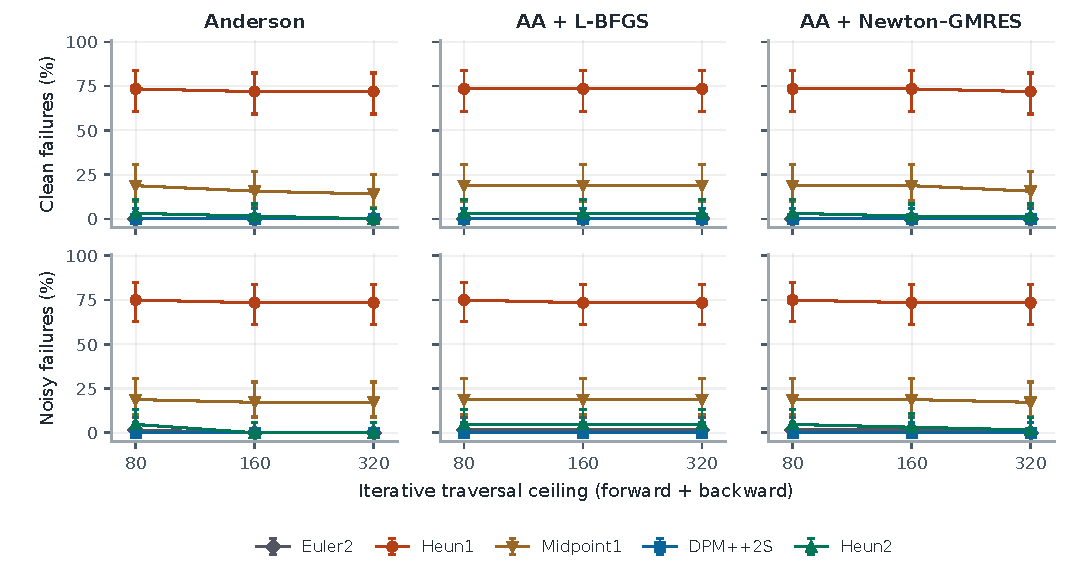
\includegraphics[width=.9\linewidth]{../figures/controls.pdf}
\caption{Observed failure percentages across the three registered iterative ceilings. Columns use different inverse procedures on the same 64 reused primary seeds. Rows use the paired target arms. Bars are two-sided exact binomial 95\% intervals. Coincident curves indicate identical displayed outcomes.}
\label{fig:controls}
\end{figure}

\begin{table}[H]
\centering\small
\begin{tabular}{@{}lllrrrrr@{}}\toprule
Cohort & Map & Target & Failures & Mean $e_x$ & Mean $e_y$ & Mean $e_{\rm flow}$ & Mean $N_f$\\\midrule
\tablerows{../manuscript/generated/fresh_rows}
\bottomrule\end{tabular}
\caption{Separately frozen VE and FFHQ64 cohorts at the 160-forward AA ceiling. The forward reference is clean and shared across target arms within each map. Iterative forwards exclude initialization and diagnostics.}
\label{tab:fresh}
\end{table}

\FloatBarrier
\section{Timing, precision and higher-work diagnostics}
\label{sec:diagnostics}
\paragraph{Contiguous wall time and device change.}
\Cref{tab:wall} starts its timer before initialization. The maximum observed overrun is \WallOverrun{}\,s. The charged forward count includes the late call when one occurs. The primary GPU target and the CPU evaluation of the source can disagree at the scale of the stopping tolerance. \Cref{tab:precision} pairs the 160-forward primary clean prefixes with fresh CPU targets on the same primary states. All \PrecisionFlags{} flags agree. Both studies are repeated controls on the same seeds. The release also gives all 10\,s and 20\,s primary component prefixes, with initialization separate and the original 320-traversal outer cap flagged when it censors an arm.

\begin{table}[htbp]
\centering\small
\begin{tabular}{@{}lrrrrrr@{}}\toprule
& \multicolumn{2}{c}{Failures} & \multicolumn{2}{c}{Mean elapsed (s)} & \multicolumn{2}{c}{Mean charged forwards}\\
\cmidrule(lr){2-3}\cmidrule(lr){4-5}\cmidrule(l){6-7}
Map & Clean & Noisy & Clean & Noisy & Clean & Noisy\\\midrule
\tablerows{../manuscript/generated/wall_rows}
\bottomrule\end{tabular}
\caption{Actual 20\,s contiguous Anderson allocation on the reused primary cohort. Elapsed time and charged calls include initialization and overrun. Final verification is outside the allocation.}
\label{tab:wall}
\end{table}

\begin{table}[htbp]
\centering\small
\begin{tabular}{@{}lrrrrr@{}}\toprule
Map & GPU-target fail. & CPU-target fail. & CPU mean $e_x$ & CPU mean $e_y$ & CPU mean $N_f$\\\midrule
\tablerows{../manuscript/generated/precision_rows}
\bottomrule\end{tabular}
\caption{Clean targets on the same primary sources with AA160. The inverse uses the CPU operator in both columns. CPU metrics use targets generated by that same operator.}
\label{tab:precision}
\end{table}

\paragraph{Compression on low-residual Heun1 misses.}
Let $y=F_{\rm GPU}(x)$ be the saved clean target and $\widehat x$ the iterate selected using the CPU residual. For the \PrimaryHeunOneLowResidual{} source misses at AA320 with $e_y<2\times10^{-6}$, we computed the upper bound
\[
 \frac{\rms(F_{\rm CPU}(\widehat x)-F_{\rm CPU}(x))}{\rms(\widehat x-x)}
 \le \frac{e_y+\rms(F_{\rm GPU}(x)-F_{\rm CPU}(x))}{e_x}.
\]
The largest right-hand side across these pairs is at most \PrimarySecantUpper{}. The denominator uses the actual source error for each seed. The worst clean Heun1 CPU--GPU mismatch over the primary panel reaches \TargetMismatch{}. These ratios are finite-displacement bounds consistent with severe inverse sensitivity. Exact root multiplicity and local Jacobian singular values are separate properties. The same-device replay checks AA160 flags, while this compression bound uses the original AA320 run.

\paragraph{Geometric Heun4.}
This controlled repeat uses the four substeps from the structural limit and the original paired primary noise realization. It costs eight denoiser calls per map. \Cref{tab:heun4,tab:cpu-fidelity} report its recovery and the consistent CPU forward reference comparison. At the smallest ceilings the inverse has fewer candidate evaluations, even though forward RMS improves. The model is the same learned checkpoint throughout.

\begin{table}[htbp]
\centering\small
\begin{tabular}{@{}rlrrrr@{}}\toprule
Ceiling & Target & Failures & Mean $e_x$ & Mean $e_y$ & Mean $N_f$\\\midrule
\tablerows{../manuscript/generated/heun_four_rows}
\bottomrule\end{tabular}
\caption{Geometric Heun4, both target arms, reused primary 64. Forward calls are counted per inverse and exclude initialization and diagnostics.}
\label{tab:heun4}
\end{table}

\begin{table}[htbp]
\centering\small
\begin{tabular}{@{}lrr@{}}\toprule
Map & CPU mean $e_{\rm flow}$ & 95\% seed-bootstrap interval\\\midrule
\tablerows{../manuscript/generated/fidelity_cpu_rows}
\bottomrule\end{tabular}
\caption{Same-device forward fidelity on the primary 64 sources. All maps and Heun128 are regenerated on CPU.}
\label{tab:cpu-fidelity}
\end{table}

\paragraph{Native optimizer stress test.}
The first eight primary indices are fixed before running this diagnostic. For their regenerated clean CPU targets, run AA with up to 80 forwards followed by PyTorch L-BFGS with strong-Wolfe search, history 20, learning rate 1, gradient tolerance $10^{-13}$ and change tolerance $10^{-18}$. The continuation may evaluate up to 500 closures and uses the same $2\times10^{-6}$ residual stop. Every closure uses one map forward and one map backward, including evaluations spent in the line search. The native optimizer can stop earlier. \Cref{tab:native} reports the actual counts. This uses unequal compute across maps and is a restricted optimization control. Hong et al.~\cite{hong2024} use different optimizers, map variants and application protocols.

\begin{table}[htbp]
\centering\small
\begin{tabular}{@{}lrrrrrr@{}}\toprule
Map & Failures & Mean $e_x$ & Mean $e_y$ & Mean $N_f$ & Mean $N_b$ & Mean closures\\\midrule
\tablerows{../manuscript/generated/native_rows}
\bottomrule\end{tabular}
\caption{Native L-BFGS diagnostic on eight fixed-index reused sources. The forward count includes the AA warm work. Initialization, target generation and final diagnostics are separate.}
\label{tab:native}
\end{table}

\FloatBarrier
\paragraph{Recovered source arrays.}
\Cref{fig:gallery} uses the first two latent indices from each of primary CIFAR-VP and FFHQ64. The plotted arrays are the saved returned states and the generating source. The target differs by map, since each inverse receives its own map's output. Source states at sigma 2 contain substantial noise.

\begin{figure}[htbp]
\centering
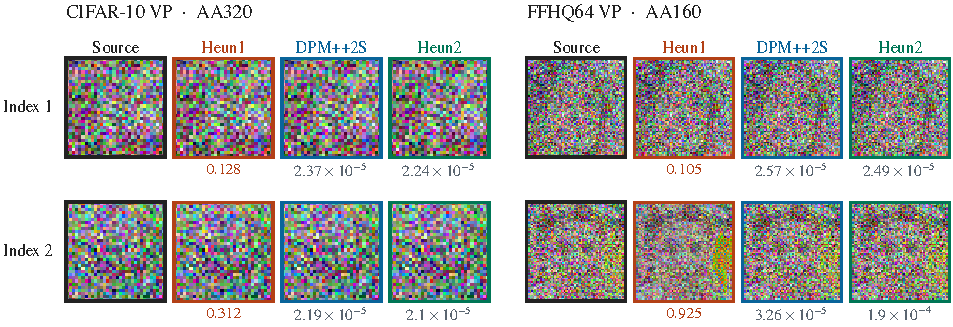
\includegraphics[width=\linewidth]{../figures/recovery_gallery.pdf}
\caption{Saved clean-target inverse states on the first two indices of each shown cohort, at the respective headline AA ceilings of \PrimaryCap{} and \FFHQCap{}. All tiles share the $[-4,4]$ display mapping to retain contrast in the noisy states. Numbers beneath the reconstructions are $e_x$ on the unclipped arrays. These are learned-model interval states.}
\label{fig:gallery}
\end{figure}

\paragraph{Earlier scientific controls.}
An exact 50,000-atom CIFAR training-image prior produced two Heun1 failures on 32 sources in an earlier controlled numerical experiment. This prior memorizes its atoms. Four selected full $3072$-dimensional neural Jacobians had Heun1 minimum singular values of approximately $0.00091$--$0.00419$, versus $0.05447$--$0.06045$ for DPM++2S. The Jacobians overlap the earlier VP cohort and measure local conditioning. The inherited directional response selector used 36 denoiser evaluations versus eight for a cheaper Heun2 response baseline and did not establish an acceleration benefit. Source-sketch controls received extra information and did not show a material gain. The earlier privileged noisy-target initializer received the clean output. Only the corrected target-only protocol informs the reported noisy-target recovery claims.

\FloatBarrier
\section{Controlled family ablation}
\label{sec:controlled}

\paragraph{Frozen design.}
We froze the public EDM FFHQ64-VP checkpoint, two intervals, the weight grid and \SweepN{} consecutive latent seeds starting at 2069020000. Both intervals have $r=1/16$ and $q=\kappa=1/4$. The sources and endpoints stay fixed within each block. With second evaluation at $a/4$, varying $w_1$ and setting $w_2=15/16-w_1$ gives $F_{w_1}(x)=F_0(x)+w_1[D_a(x)-D_{a/4}(p_a(x))]$. The zero arm is log-SNR midpoint DPM++2S. The most negative arm transfers Heun1's weight to the same midpoint stage.

\paragraph{Targets, reference and cost.}
For each seed and block we draw the same seeded float32 standard Gaussian array, promote it to float64, multiply by $80$, and generate the block's source with Heun64 from 80 to $a$. The same draw gives a matched seed across blocks, with different source states. Each arm uses its own clean output $y$ and initializes with two reverse Euler calls from $y$. It uses the same residual-selected Anderson recurrence as Supplement~D, with memory five, damping $0.8$, ridge $10^{-5}$, residual stop $2\times10^{-6}$ and a ceiling of 160 iterative forwards. A recovered source has $e_x\le0.02$. Heun128 from the same source on the same interval is the common forward reference for all arms of a block. Source, initializer and reference grids use power 7. The same device evaluates targets, inverses, references and probes, with single-image float32 denoiser evaluation on an H200, TF32 disabled and float64 outer states. The original FFHQ64 and CIFAR panels use their separate registered devices and seeds.

\paragraph{Local response.}
At source $x$, for a direction $v$ normalized to $\rms(v)=1$, evaluate the centered directional gain
\[
 g_v(x)=\frac{\rms(F(x+10^{-3}v)-F(x-10^{-3}v))}{2\cdot10^{-3}}.
\]
We draw four independent coordinatewise Rademacher directions per seed and use those same directions for all weights and both blocks. The table gives the seed median of each seed's smallest gain among those four directions, $g_{\rm rand}$. A separate diagnostic, $g_{\rm err}$, uses the unit-RMS direction from $x$ to the selected $\widehat x$ if $e_x>10^{-8}$. That direction depends on the inverse outcome and is used only after inversion. These finite differences sample directional sensitivity at the source. A large gain along sampled directions still permits small gains in other directions. The measurements are neither minimum singular values nor bounds on the full inverse condition number.

\begin{table}[H]
\centering\small
\setlength{\tabcolsep}{4.5pt}
\begin{tabular}{@{}lrrrrrrrrr@{}}\toprule
Interval & $w_1$ & $w_2$ & Recovered & Mean $e_x$ & Mean $e_y$ & Mean $e_{\rm flow}$ & Mean $N_f$ & $g_{\rm rand}$ & $g_{\rm err}$\\
\midrule
\tablerows{../manuscript/generated/sweep_rows}
\bottomrule
\end{tabular}
\caption{All frozen arms of the controlled learned-model family ablation. $N_f$ is iterative work per inverse. Each arm and seed has two target, two initialization and two final residual calls outside the cap. Centered probes use four calls per direction. Gain columns report medians across seeds. The \SweepRows{} arm outcomes are nested within \SweepN{} matched latent seeds.}
\label{tab:controlled}
\end{table}

\begin{table}[H]
\centering\small
\setlength{\tabcolsep}{6pt}
\begin{tabular}{@{}lrrrrrrr@{}}\toprule
Interval & $w_1$ & Gains & Losses & Mean $\Delta N_f$ & Range of $\Delta N_f$ & Mean $\Delta e_{\rm flow}$ & Mean $\Delta g_{\rm rand}$\\
\midrule
\tablerows{../manuscript/generated/sweep_paired}
\bottomrule
\end{tabular}
\caption{Paired comparisons with $w_1=0$ within each block. Gains and losses are recovery discordances. Changes are arm minus zero for the same seed. Ranges describe the observed differences.}
\label{tab:controlled-paired}
\end{table}

\begin{figure}[htbp]
\centering
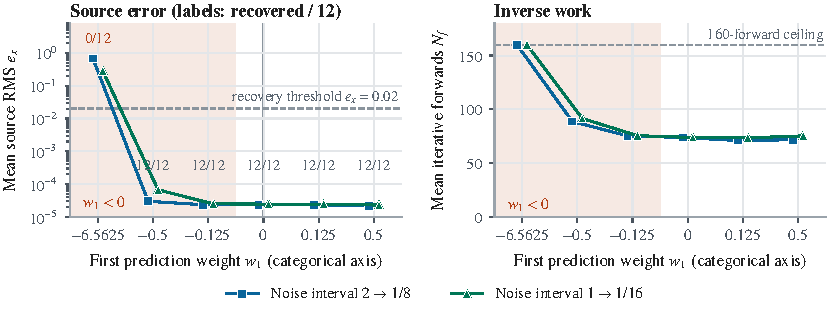
\includegraphics[width=.55\linewidth]{../figures/controlled.pdf}
\caption{The full controlled sweep on both fixed-ratio intervals (main paper Fig.~3). The weight axis is categorical; panels (a) and (c) use log scales. Numbers above (a) count recovered sources and apply to both blocks. Attained residuals and $g_{\rm err}$ are in \cref{tab:controlled}.}
\label{fig:controlled}
\end{figure}

Each of the five tested weights between $-0.5$ and $0.5$ recovers all twelve sources in both blocks. At $w_1=-0.5$ on $2\to1/8$, mean forward RMS drops from $0.0460$ to $0.0347$ relative to zero, with $14.8$ more mean iterative calls. The lower-noise block shows the same trade-off. The $-6.5625$ arm reaches the ceiling on every source and recovers none in either block. Its median $g_{\rm rand}$ is larger than at zero in both blocks.

Each arm uses its own output and target-based initializer. Across blocks, source states and absolute noise scales vary together. The Heun64/128 mean RMS differences are $1.89\times10^{-5}$ and $1.28\times10^{-5}$ for $2\to1/8$ and $1\to1/16$. The sweep used 29,120 forwards, including 13,082 iterative calls and the remaining calls for qualification, generation, references, initialization and diagnostics.
\FloatBarrier

\section{Reproduction and scope}
\label{sec:replay}
\paragraph{What is counted.}
The unit is a latent seed. \Cref{tab:physical} enumerates the \NestedRecords{} terminal records and corresponding physical denoiser traversals of the seven completed panels, including generation and checks where executed. Counts for shared warm starts differ from their per-arm charged work. Historical generation of the primary GPU targets precedes these seven panels. The primary diagnostics reuse the same sources, with the native check using only their first eight indices. Inference records and prefix observations are nested and the distinct checkpoint cohorts stay separate.

\begin{table}[htbp]
\centering\small
\begin{tabular}{@{}lrrr@{}}\toprule
Panel & Terminal records & Physical forwards & Physical backwards\\\midrule
\tablerows{../manuscript/generated/physical_rows}
\bottomrule\end{tabular}
\caption{Physical counts reconciled from the recorded per-block counters and component work. Each forward count is an image-level denoiser evaluation. The elapsed-time arm charges late evaluations even when their candidate is ineligible.}
\label{tab:physical}
\end{table}

\paragraph{Replay.}
The evidence archive regenerates summaries and plots offline from saved traces and figure arrays. Full state tensors supply a separate check of terminal RMS values, including the controlled sweep. Recorded residuals agree with terminal diagnostics. The archive includes the frozen configurations, checkpoint hashes, figure provenance and bounded inference commands.

The two-image example uses CIFAR-10 arrays and a specified exact prior. The learned experiments use public checkpoints and numerical states, with no new physical acquisitions, training or recruited participants. Source error and reference fidelity are pixel-coordinate RMS for the numerical task. Our study leaves perceptual image quality, editing behavior and demographic claims outside its evaluation. The measured finite-budget failures cannot determine whether a learned map has multiple preimages.

\FloatBarrier
\section*{LLM Usage Statement}
The main paper's LLM Usage Statement covers the study and this supplement.
{\small\bibliographystyle{ieeenat_fullname}\bibliography{references}}
\end{document}
